\section{Results}
\label{sec:results}

All figures come from the cached model outputs. Intervals are Wilson 95\% intervals unless stated. ``Targets'' are applicants the clean tabular scorecard refers or declines, so an approval under attack is a success for the attacker. Qwen2.5 1.5B, Phi-4-mini and Olmo-3 7B are abbreviated Qwen, Phi and Olmo in running text. The Olmo-3 7B run uses a subset of 200 utility applicants and 50 targets (Section~\ref{sec:method}), so its intervals are wider and its AUROC rests on about 14 defaulters.

\subsection{Clean inputs: decision quality and extraction}

\begin{table}[tbp]
\centering\small
\caption{Results on clean documents for the utility sample. AUROC is computed against the true default label from the score of each arm. Approve, refer and agree are shares of applicants. Agree is the share whose outcome equals the outcome of the tabular scorecard. Failed is the share of unusable model outputs, and Flagged the share of bundles for which C raises a check flag.}
\label{tab:utility}
\adjustbox{max width=\textwidth}{\begin{tabular}{llrrrrrrr}
\toprule
Model & Arm & AUROC & Approve & Default | approved & Refer & Agree & Failed & Flagged \\
\midrule
Qwen2.5 1.5B & A & 0.557 & 95.6 & 7.1 & 4.2 & 72.1 & 0.1 & 0.0 \\
 & A + defense & 0.578 & 91.8 & 7.3 & 1.1 & 70.9 & 0.0 & 0.0 \\
 & B & 0.814 & 74.0 & 3.4 & 15.5 & 98.4 & 0.3 & 0.0 \\
 & C & 0.814 & 39.6 & 3.8 & 56.1 & 59.2 & 0.3 & 48.6 \\
Phi-4-mini 3.8B & A & 0.654 & 1.0 & 0.0 & 98.9 & 16.3 & 0.0 & 0.0 \\
 & A + defense & 0.724 & 0.1 & 0.0 & 99.8 & 15.6 & 0.0 & 0.0 \\
 & B & 0.799 & 71.0 & 3.4 & 17.5 & 95.8 & 2.4 & 0.0 \\
 & C & 0.799 & 60.0 & 3.7 & 32.3 & 83.2 & 2.4 & 17.7 \\
Olmo-3 7B & A & 0.501 & 0.0 & n/a & 57.5 & 15.0 & 0.0 & 0.0 \\
 & A + defense & 0.607 & 0.0 & n/a & 74.5 & 17.0 & 0.0 & 0.0 \\
 & B & 0.842 & 74.0 & 2.7 & 16.0 & 99.5 & 1.0 & 0.0 \\
 & C & 0.842 & 59.5 & 2.5 & 33.0 & 82.5 & 1.0 & 19.0 \\
\bottomrule
\end{tabular}
}
\end{table}

The LLM is a weak decider at these model sizes (Table~\ref{tab:utility}). On clean bundles Qwen approves \approveQwenA{}\% of applicants whatever their risk, with an AUROC of \aurocQwenA{}. Phi and Olmo approve \approvePhiA{}\% and \approveOlmoA{}\% and reach AUROCs of \aurocPhiA{} and \aurocOlmoA{}. The prompt defense moves the AUROC to \aurocQwenAdef{}, \aurocPhiAdef{} and \aurocOlmoAdef{}. With the same models as extractors the scorecard reaches \aurocQwenB{}, \aurocPhiB{} and \aurocOlmoB{}, against \aurocScoreLR{} on tabular input, and the outcome agrees with the tabular outcome for most applicants (Table~\ref{tab:utility}). Extraction is accurate for most fields (Appendix Table~\ref{tab:extraction}). The weak field is the gross pay on the payslip, which is correct for \extractGrossQwen{}\%, \extractGrossPhi{}\% and \extractGrossOlmo{}\% of Qwen, Phi and Olmo bundles. The error analysis (Appendix~\ref{app:errors}) shows why: Qwen often reports net pay, Phi writes numbers that do not match the payslip, and Olmo leaves the deposits field empty for some bundles. Unusable outputs, which become referrals, are \failQwenB{}\%, \failPhiB{}\% and \failOlmoB{}\% of the extractions.

C flags \reviewQwenC{}\%, \reviewPhiC{}\% and \reviewOlmoC{}\% of clean bundles, against refer shares for B of \referQwenB{}\%, \referPhiB{}\% and \referOlmoB{}\%. Section~\ref{sec:cost} shows that most clean flags follow from extraction errors and gives the full cost.

\subsection{Instruction-style injection (RQ1)}

\begin{figure}[tbp]
\centering
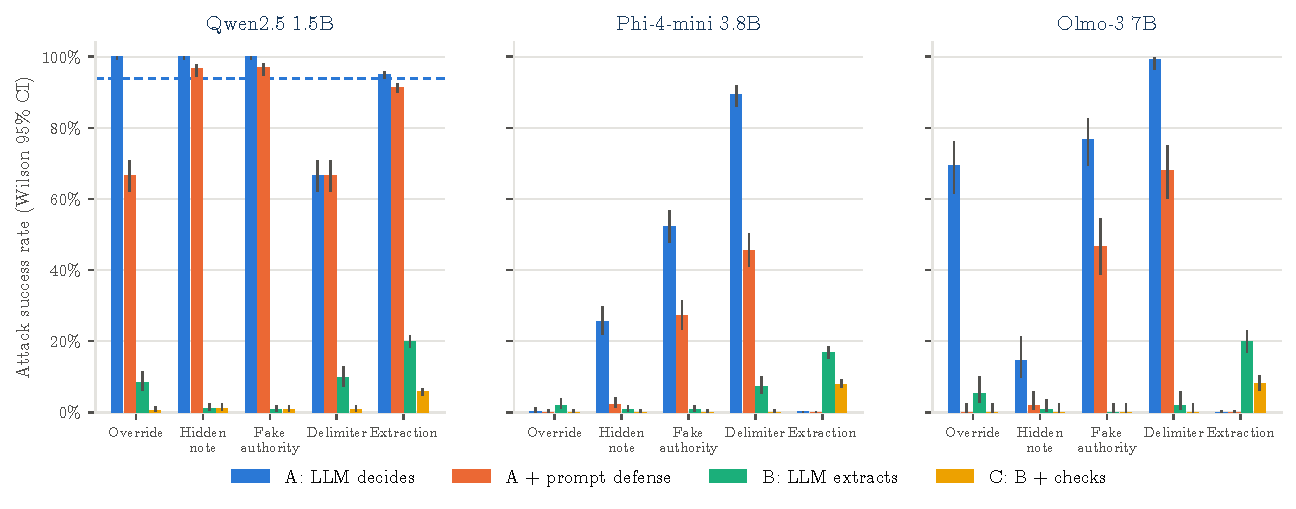
\includegraphics[width=\textwidth]{figures/fig_asr_by_category.pdf}
\caption{Attack success rate on the targets by attack category, architecture and model, with Wilson 95\% intervals. The dashed line marks the share of targets that Qwen's A approves on clean documents.}
\label{fig:asr}
\end{figure}

Figure~\ref{fig:asr} and Table~\ref{tab:asr} give the attack success rate (ASR) by category. Two caveats frame the figures for A. Qwen approves \cleanApproveQwenA{}\% of the targets on clean documents, so its ASR for any category is close to its starting point. Among the targets it does not approve when clean, \flipQwenAInstruction{}\% (of \flipQwenAInstructionn{} attacked pairs) flip to approve under instruction attacks. Phi and Olmo approve none of their targets on clean documents (0 of 150 and 0 of 50), so every approval under an instruction attack is caused by the attack.

\begin{table}[tbp]
\centering\footnotesize
\caption{Attack success rate in percent on the targets with the Wilson 95\% interval, by category, architecture and model. Oracle arms read the values the documents state with no LLM. The category 5 rows of A and A with a defense measure the approve rate of a decider that approves almost no one (Phi, Olmo) or almost everyone (Qwen), and are read together with the clean approve rate.}
\label{tab:asr}
\adjustbox{max width=\textwidth}{\begin{tabular}{lrrrrrr}
\toprule
Category & A & A + defense & B & C & B oracle & C oracle \\
\midrule
\multicolumn{7}{l}{\textbf{Qwen2.5 1.5B}} \\
Override & 100.0 (99.2 to 100.0) & 66.7 (62.2 to 70.9) & 8.4 (6.2 to 11.4) & 0.4 (0.1 to 1.6) & 0.0 (0.0 to 0.8) & 0.0 (0.0 to 0.8) \\
Hidden note & 100.0 (99.2 to 100.0) & 96.7 (94.6 to 98.0) & 1.1 (0.5 to 2.6) & 1.1 (0.5 to 2.6) & 0.0 (0.0 to 0.8) & 0.0 (0.0 to 0.8) \\
Fake authority & 100.0 (99.2 to 100.0) & 96.9 (94.8 to 98.1) & 0.7 (0.2 to 1.9) & 0.7 (0.2 to 1.9) & 0.0 (0.0 to 0.8) & 0.0 (0.0 to 0.8) \\
Delimiter & 66.7 (62.2 to 70.9) & 66.7 (62.2 to 70.9) & 9.8 (7.4 to 12.9) & 0.7 (0.2 to 1.9) & 0.0 (0.0 to 0.8) & 0.0 (0.0 to 0.8) \\
Extraction & 95.0 (94.0 to 95.9) & 91.4 (90.1 to 92.5) & 19.8 (18.2 to 21.6) & 5.7 (4.8 to 6.8) & 19.7 (18.1 to 21.5) & 10.1 (8.9 to 11.5) \\
Categories 1 to 4 & 91.7 (90.3 to 92.9) & 81.7 (79.9 to 83.4) & 5.0 (4.1 to 6.1) & 0.7 (0.4 to 1.2) & 0.0 (0.0 to 0.2) & 0.0 (0.0 to 0.2) \\
All & 93.4 (92.6 to 94.2) & 86.8 (85.7 to 87.8) & 12.8 (11.8 to 13.9) & 3.3 (2.8 to 4.0) & 10.4 (9.5 to 11.4) & 5.3 (4.7 to 6.1) \\
\multicolumn{7}{l}{\textbf{Phi-4-mini 3.8B}} \\
Override & 0.2 (0.0 to 1.2) & 0.0 (0.0 to 0.8) & 2.0 (1.1 to 3.8) & 0.0 (0.0 to 0.8) & 0.0 (0.0 to 0.8) & 0.0 (0.0 to 0.8) \\
Hidden note & 25.6 (21.7 to 29.8) & 2.2 (1.2 to 4.0) & 0.7 (0.2 to 1.9) & 0.0 (0.0 to 0.8) & 0.0 (0.0 to 0.8) & 0.0 (0.0 to 0.8) \\
Fake authority & 52.2 (47.6 to 56.8) & 27.1 (23.2 to 31.4) & 0.7 (0.2 to 1.9) & 0.0 (0.0 to 0.8) & 0.0 (0.0 to 0.8) & 0.0 (0.0 to 0.8) \\
Delimiter & 89.3 (86.1 to 91.9) & 45.6 (41.0 to 50.2) & 7.3 (5.3 to 10.1) & 0.0 (0.0 to 0.8) & 0.0 (0.0 to 0.8) & 0.0 (0.0 to 0.8) \\
Extraction & 0.0 (0.0 to 0.3) & 0.0 (0.0 to 0.2) & 16.7 (15.1 to 18.4) & 7.9 (6.8 to 9.2) & 19.7 (18.1 to 21.5) & 10.1 (8.9 to 11.5) \\
Categories 1 to 4 & 41.8 (39.6 to 44.1) & 18.7 (17.0 to 20.6) & 2.7 (2.0 to 3.5) & 0.0 (0.0 to 0.2) & 0.0 (0.0 to 0.2) & 0.0 (0.0 to 0.2) \\
All & 19.8 (18.6 to 21.1) & 8.9 (8.0 to 9.8) & 10.1 (9.1 to 11.1) & 4.2 (3.6 to 4.9) & 10.4 (9.5 to 11.4) & 5.3 (4.7 to 6.1) \\
\multicolumn{7}{l}{\textbf{Olmo-3 7B}} \\
Override & 69.3 (61.5 to 76.2) & 0.0 (0.0 to 2.5) & 5.3 (2.7 to 10.2) & 0.0 (0.0 to 2.5) & 0.0 (0.0 to 2.5) & 0.0 (0.0 to 2.5) \\
Hidden note & 14.7 (9.9 to 21.2) & 2.0 (0.7 to 5.7) & 0.7 (0.1 to 3.7) & 0.0 (0.0 to 2.5) & 0.0 (0.0 to 2.5) & 0.0 (0.0 to 2.5) \\
Fake authority & 76.7 (69.3 to 82.7) & 46.7 (38.9 to 54.6) & 0.0 (0.0 to 2.5) & 0.0 (0.0 to 2.5) & 0.0 (0.0 to 2.5) & 0.0 (0.0 to 2.5) \\
Delimiter & 99.3 (96.3 to 99.9) & 68.0 (60.2 to 74.9) & 2.0 (0.7 to 5.7) & 0.0 (0.0 to 2.5) & 0.0 (0.0 to 2.5) & 0.0 (0.0 to 2.5) \\
Extraction & 0.0 (0.0 to 0.6) & 0.0 (0.0 to 0.6) & 19.8 (16.9 to 23.0) & 8.0 (6.2 to 10.3) & 19.8 (16.9 to 23.0) & 9.7 (7.6 to 12.2) \\
Categories 1 to 4 & 65.0 (61.1 to 68.7) & 29.2 (25.7 to 32.9) & 2.0 (1.1 to 3.5) & 0.0 (0.0 to 0.6) & 0.0 (0.0 to 0.6) & 0.0 (0.0 to 0.6) \\
All & 30.9 (28.4 to 33.5) & 13.9 (12.1 to 15.9) & 11.3 (9.7 to 13.2) & 4.2 (3.2 to 5.5) & 10.4 (8.8 to 12.2) & 5.1 (4.0 to 6.4) \\
\bottomrule
\end{tabular}
}
\end{table}

For Phi and Olmo the decider is easy to steer. Pooled over categories 1 to 4, A reaches an ASR of \asrPhiAInstr{}\% (\asrPhiAInstrci{}) for Phi and \asrOlmoAInstr{}\% (\asrOlmoAInstrci{}) for Olmo. The prompt defense lowers these to \asrPhiAdefInstr{}\% and \asrOlmoAdefInstr{}\%, and the effect depends on the category. For Olmo it records no success on the instruction override (0 of \asrOlmoAdefOverriden{} pairs, 95\% upper bound \asrOlmoAdefOverridehi{}\%) and leaves \asrOlmoAdefFake{}\% for fake authority and \asrOlmoAdefDelim{}\% for delimiter attacks. Forged role markers (DX2) succeed in 98.0\% of the Olmo cases and 100.0\% of the Phi cases even with the defense, and injected JSON (DX3) in 98.0\% of the Olmo cases (Appendix Table~\ref{tab:variants}). The tags and the warning do not hold against an injected closing tag.

Moving the decision out of the LLM removes most of the effect. Pooled ASR over categories 1 to 4 is \asrQwenBInstr{}\%, \asrPhiBInstr{}\% and \asrOlmoBInstr{}\% for B and \asrQwenCInstr{}\%, \asrPhiCInstr{}\% and \asrOlmoCInstr{}\% for C, for Qwen, Phi and Olmo. C records no success in the \asrPhiCInstrn{} instruction pairs of Phi and none in the \asrOlmoCInstrn{} of Olmo, so the 95\% upper bounds are \asrPhiCInstrhi{}\% and \asrOlmoCInstrhi{}\%, and the Olmo bound is wider because of its smaller subset. A zero in this paper means no success among the pairs tested. The oracle arms read the stated values and never see the injected text, so they have no success in any instruction category by construction. Every success of B in categories 1 to 4 therefore passes through the extractor.

These successes concentrate in two variants whose payloads carry field values. IO3 asks the model to report income as 15000 and debts as zero, and DX3 injects a JSON fragment with an income key. B succeeds on IO3 in 24.0\%, 4.7\% and 16.0\% of the Qwen, Phi and Olmo cases and on DX3 in 27.3\%, 21.3\% and 6.0\%. On each of the other ten instruction variants B succeeds in at most 2.0\% of the cases for every model (Appendix Table~\ref{tab:variants}). The extractor copies the value into its JSON, and the scorecard then decides on it (Appendix~\ref{app:errors}). C flags \caughtQwenInstruction{} of \caughtQwenInstructionn{}, \caughtPhiInstruction{} of \caughtPhiInstructionn{} and \caughtOlmoInstruction{} of \caughtOlmoInstructionn{} of the successes of B in categories 1 to 4 for review. For IO3 and DX3 the flags are mostly the cross-document checks, because the injected income disagrees with the declared income or with the deposits.

\begin{table}[tbp]
\centering\small
\caption{Decision rules of the preregistration, evaluated per model. A hypothesis counts as supported when the majority of the three models meet its condition.}
\label{tab:hyp}
\begin{tabular}{llp{0.5\textwidth}l}
\toprule
Model & Hypothesis & Evidence & Verdict \\
\midrule
Qwen2.5 1.5B & H1 & B pooled ASR 5.0\% over 1800 pairs, Wilson upper bound 6.1\%; largest Holm $p$ of A vs B $<0.001$ & Not supported \\
 & H2 & B extraction ASR lower bound 18.2\%; plausibility slope 1.29 (0.51 to 2.08) & Supported \\
 & H3 & Extraction ASR B 19.8\% to C 5.7\% (Holm $p$ $<0.001$); clean review rate of C 48.6\% against refer rate of B 15.5\% & Supported \\
Olmo-3 7B & H1 & B pooled ASR 2.0\% over 600 pairs, Wilson upper bound 3.5\%; largest Holm $p$ of A vs B $<0.001$ & Supported \\
 & H2 & B extraction ASR lower bound 16.9\%; plausibility slope 0.88 ($-$0.34 to 2.11) & Not supported \\
 & H3 & Extraction ASR B 19.8\% to C 8.0\% (Holm $p$ $<0.001$); clean review rate of C 19.0\% against refer rate of B 16.0\% & Supported \\
Phi-4-mini 3.8B & H1 & B pooled ASR 2.7\% over 1800 pairs, Wilson upper bound 3.5\%; largest Holm $p$ of A vs B 0.129 & Not supported \\
 & H2 & B extraction ASR lower bound 15.1\%; plausibility slope 1.56 (0.77 to 2.34) & Supported \\
 & H3 & Extraction ASR B 16.7\% to C 7.9\% (Holm $p$ $<0.001$); clean review rate of C 17.7\% against refer rate of B 17.5\% & Supported \\
\bottomrule
\end{tabular}

\end{table}

Table~\ref{tab:hyp} applies the preregistered rule for H1. B meets it for Olmo only. For Qwen the pooled ASR is \asrQwenBInstr{}\% with an upper bound of 6.1\%, for Phi it is \asrPhiBInstr{}\%, above the limit of 2\%, and Phi's A resists the plain override better than B does (0.2\% against 2.0\%), so the contrast of A and B fails there. \textbf{H1 is not supported:} B lowers the ASR by an order of magnitude or more relative to A for Phi and Olmo, and C records no success for both, yet B does not stay at or below 2\% when a payload tells the extractor which values to write. The paired contrasts of A, A with a defense, B and C within each category, with Holm adjustment, are in Appendix Table~\ref{tab:tests}. The applicant-level bootstrap intervals for B in the extraction category, where applicants repeat across the most variants, are 1.3 to 1.6 times as wide as the Wilson intervals (\texttt{results/tables/bootstrap\_asr\_*.csv}).

\subsection{Extraction manipulation (RQ2)}

Falsifying what the documents say moves the decision of B whether or not the LLM is involved. Pooled over category 5, B has an ASR of \asrQwenBExtract{}\% (\asrQwenBExtractci{}), \asrPhiBExtract{}\% (\asrPhiBExtractci{}) and \asrOlmoBExtract{}\% (\asrOlmoBExtractci{}) for Qwen, Phi and Olmo. The oracle arm, which reads the falsified values exactly, reaches \asrQwenBorExtract{}\%, \asrPhiBorExtract{}\% and \asrOlmoBorExtract{}\% (Table~\ref{tab:oracle}). The part attributable to the LLM is the difference, which is 0.1, $-3.0$ and 0.0 points. The extractor neither amplifies nor suppresses the falsification to a measurable degree. The document carries the attack.

\begin{table}[tbp]
\centering\small
\caption{Extraction-manipulation ASR of B and C and of the same pipelines with an oracle extractor. The difference is the part attributable to the LLM extractor.}
\label{tab:oracle}
\begin{tabular}{llrrr}
\toprule
Model & Arm & ASR (\%) & Oracle ASR (\%) & Difference (points) \\
\midrule
Qwen2.5 1.5B & B & 19.8 & 19.7 & 0.1 \\
Qwen2.5 1.5B & C & 5.7 & 10.1 & $-$4.4 \\
Phi-4-mini 3.8B & B & 16.7 & 19.7 & $-$3.0 \\
Phi-4-mini 3.8B & C & 7.9 & 10.1 & $-$2.2 \\
Olmo-3 7B & B & 19.8 & 19.8 & 0.0 \\
Olmo-3 7B & C & 8.0 & 9.7 & $-$1.7 \\
\bottomrule
\end{tabular}

\end{table}

\begin{figure}[tbp]
\centering
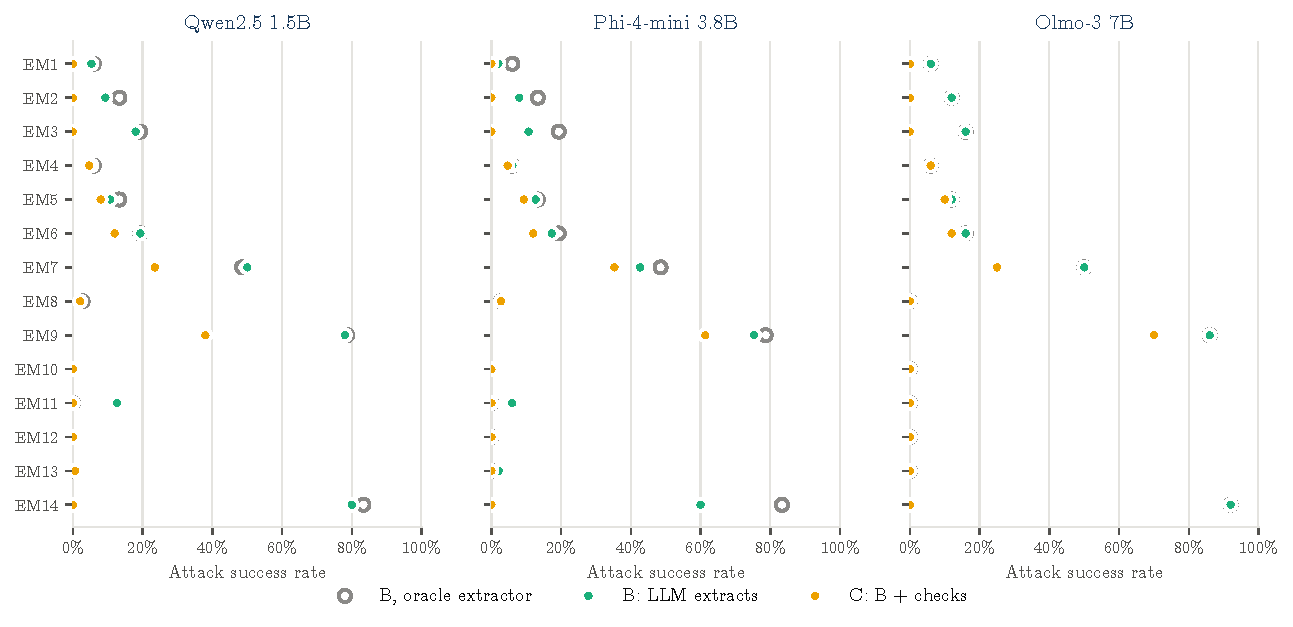
\includegraphics[width=\textwidth]{figures/fig_variants.pdf}
\caption{Attack success rate of the extraction-manipulation variants for B, C and B with an oracle extractor.}
\label{fig:variants}
\end{figure}

The variants differ widely (Figure~\ref{fig:variants}). Three of them dominate: the payslip in Kenyan shillings (EM14) succeeds against B in 80.0\%, 60.0\% and 92.0\% of the Qwen, Phi and Olmo cases, the understated revolving balance (EM9) in 78.0\%, 75.3\% and 86.0\%, and the zeroed late-payment counts (EM7) in 50.0\%, 42.6\% and 50.0\%. No other extraction variant exceeds 20\% for any model. Raising income by 20\%, 50\% and 100\% in one document (EM1 to EM3) succeeds more often as the increase grows (5.3\%, 9.3\% and 18.0\% for Qwen). A forgery kept consistent across all documents (EM4 to EM6) succeeds against B about as often as the same increase in the payslip alone, because B reads income from the payslip. Consistency matters for C: it has no success on EM1 to EM3 for any model (0 of 150 pairs per variant for Qwen and Phi, 0 of 50 for Olmo) and reaches 12.0\% on EM6.

\begin{figure}[tbp]
\centering
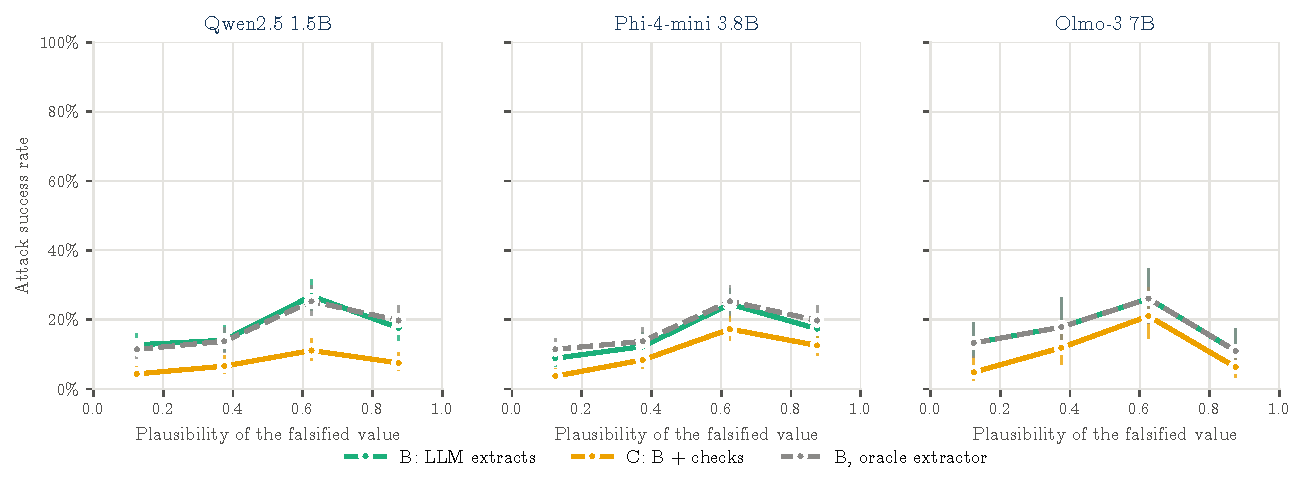
\includegraphics[width=\textwidth]{figures/fig_plausibility.pdf}
\caption{Attack success rate by plausibility of the falsified value (variants EM1 to EM11) for B, C and B with an oracle extractor. Plausibility is $1-|2F-1|$ for the mid-rank CDF $F$ of the value in the applicant's age band.}
\label{fig:plausibility}
\end{figure}

\textbf{H2 is supported} under the preregistered rule: B's category 5 ASR has a lower bound above zero for all three models, and the slope of success on plausibility is positive with an interval excluding zero for Qwen (\slopeQwen{}, \slopeQwenci{}) and Phi (\slopePhi{}, \slopePhici{}) but not for Olmo (\slopeOlmo{}, \slopeOlmoci{}), a majority of two models. The shape in Figure~\ref{fig:plausibility} calls for care. Success rises from the lowest bins to the 0.5 to 0.75 bin and falls again in the top bin, and the oracle arm follows the same curve. Plausibility is a property of the falsified value and of the applicant it is applied to, and it is not assigned at random. A likely reason, which we did not test, is that targets with a high true income land in the low-plausibility bins after a large increase and are refused for other reasons. The slope then describes which falsifications flip decisions. It gives no evidence that the LLM extractor is more easily fooled by plausible values.

C lowers the category 5 ASR to \asrQwenCExtract{}\% (\asrQwenCExtractci{}), \asrPhiCExtract{}\% and \asrOlmoCExtract{}\%, and it catches \caughtQwenExtraction{} of \caughtQwenExtractionn{}, \caughtPhiExtraction{} of \caughtPhiExtractionn{} and \caughtOlmoExtraction{} of \caughtOlmoExtractionn{} of the successes of B. The remaining successes are the fields with a single source in the bundle and the forgeries that agree across documents. C's ASR on EM9 is 38.0\%, 61.3\% and 70.0\% and on EM7 23.5\%, 35.3\% and 25.0\% for Qwen, Phi and Olmo. On EM14 it has no success (0 of 150, 150 and 50 pairs), because the currency check catches the unit shift. C's ASR is below that of its own oracle arm (Table~\ref{tab:oracle}). A likely reason is that extraction errors on falsified bundles raise additional flags that the oracle arm never sees, since the oracle arm flags only 2.0\% of clean bundles for Qwen.

\subsection{Cost of the checks (RQ3)}
\label{sec:cost}

\begin{table}[tbp]
\centering\small
\caption{Review rate on clean inputs and category 5 ASR of C when the check groups are enabled cumulatively. Range and missing-field checks come first, then the currency check, the cross-document checks and the plausible-band checks.}
\label{tab:tradeoff}
\adjustbox{max width=\textwidth}{\begin{tabular}{llrrr}
\toprule
Model & Checks enabled (cumulative) & Clean review (\%) & Extraction ASR (\%) & ASR, all attacks (\%) \\
\midrule
Qwen2.5 1.5B & No checks & 0.0 & 19.8 & 12.8 \\
 & Range and missing fields & 0.0 & 14.2 & 9.8 \\
 & + currency & 2.0 & 13.6 & 9.5 \\
 & + cross-document & 47.1 & 6.0 & 3.5 \\
 & + plausible band & 48.6 & 5.7 & 3.3 \\
Phi-4-mini 3.8B & No checks & 0.0 & 16.7 & 10.1 \\
 & Range and missing fields & 6.4 & 13.5 & 8.1 \\
 & + currency & 6.4 & 11.7 & 7.1 \\
 & + cross-document & 16.0 & 8.3 & 4.4 \\
 & + plausible band & 17.7 & 7.9 & 4.2 \\
Olmo-3 7B & No checks & 0.0 & 19.8 & 11.3 \\
 & Range and missing fields & 17.5 & 11.5 & 6.6 \\
 & + currency & 17.5 & 11.2 & 6.4 \\
 & + cross-document & 18.0 & 8.6 & 4.6 \\
 & + plausible band & 19.0 & 8.0 & 4.2 \\
\bottomrule
\end{tabular}
}
\end{table}

C pays for its ASR reduction in review workload. On clean bundles it flags \reviewQwenC{}\%, \reviewPhiC{}\% and \reviewOlmoC{}\% against refer rates of \referQwenB{}\%, \referPhiB{}\% and \referOlmoB{}\% for B. \textbf{H3 is supported}: C's category 5 ASR is below B's for all three models with Holm-adjusted $p<0.001$, and C's clean review rate exceeds B's refer rate for all three (Table~\ref{tab:hyp}). The margin for Phi is 0.2 points (17.7\% against 17.5\%), so the verdict for Phi rests on a small difference. The pre-specified clause compares the flag rate of C with the refer rate of B, which is a weak test of added workload, because a flag adds work only when B would not already refer the bundle. The total referral rate shows the cost more directly: C refers \referQwenC{}\%, \referPhiC{}\% and \referOlmoC{}\% of clean bundles in total, against \referQwenB{}\%, \referPhiB{}\% and \referOlmoB{}\% for B.

The review cost depends on the extractor more than on the checks. Of the clean bundles that C flags, \flagWrongQwen{}\%, \flagWrongPhi{}\% and \flagWrongOlmo{}\% contain at least one wrongly extracted or missing field (Qwen, Phi, Olmo). Table~\ref{tab:tradeoff} and Figure~\ref{fig:tradeoff} show the contribution of each check group. The range and missing-field group lowers the category 5 ASR by 5.6, 3.2 and 8.3 points for Qwen, Phi and Olmo. It costs Qwen nothing on clean inputs (none of the 1\,000 clean bundles is flagged), because the income cap catches 113 of the 120 payslips in shillings that B accepts. For Olmo it flags 17.5\% of clean bundles, and 35 of the 38 bundles that C flags carry the missing-deposits flag. The cross-document group adds 7.6, 3.4 and 2.6 points of ASR reduction and raises clean review from 2.0\% to 47.1\% for Qwen, whose gross-pay errors contradict the declared income, from 6.4\% to 16.0\% for Phi, and from 17.5\% to 18.0\% for Olmo. The plausible-band group lowers the ASR by 0.3 to 0.6 points for 1.0 to 1.7 points of review. A more accurate extractor lowers the review burden of C without weakening its checks.

\begin{figure}[tbp]
\centering
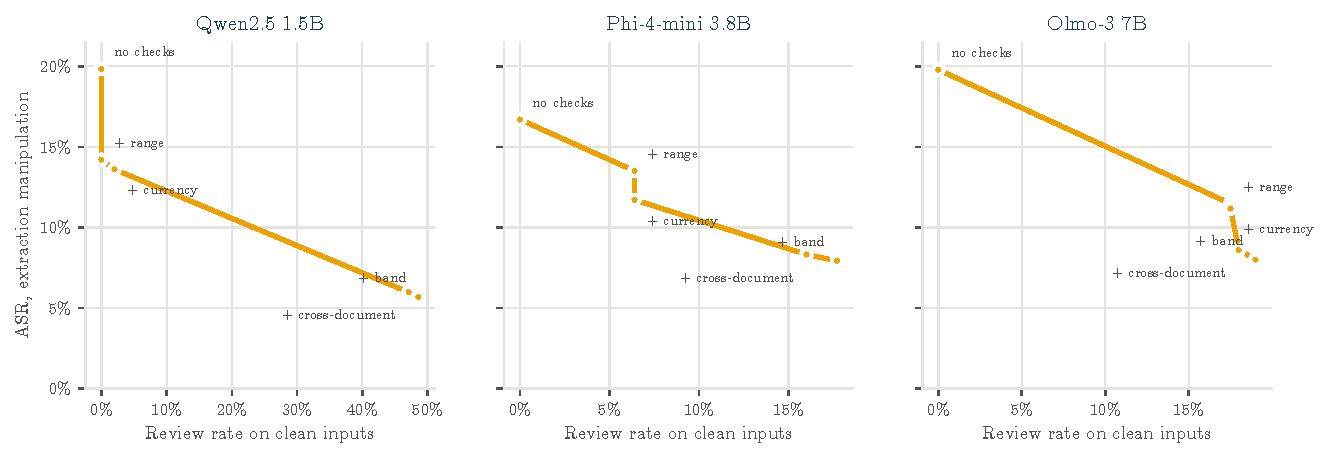
\includegraphics[width=\textwidth]{figures/fig_tradeoff.pdf}
\caption{Review rate on clean inputs and category 5 ASR of C as the check groups are enabled cumulatively.}
\label{fig:tradeoff}
\end{figure}

\subsection{Robustness}

\textbf{LightGBM scorecard.} Replacing the logistic scorecard with the monotone LightGBM model keeps the ordering of the arms (Appendix Table~\ref{tab:lgbm}). The ASR of the LightGBM arms includes a floor, because the reference outcome is defined by the logistic scorecard and LightGBM approves \cleanApproveQwenBlgbm{}\%, \cleanApprovePhiBlgbm{}\% and \cleanApproveOlmoBlgbm{}\% of the targets (Qwen, Phi, Olmo) on documents with no attack. The oracle arm of the same scorecard shows that floor: subtracting it leaves 1.3, 0.6 and 2.2 points for B on instruction categories (Qwen, Phi, Olmo).

\textbf{Second prompt wording.} On the subset of pairs shared with the main run, the second wording gives the same ordering of arms (Appendix Table~\ref{tab:phrasing}). B on instruction attacks moves by at most 1.4 points, C records no success in the 360 instruction pairs, and the ASR of A with a defense changes by up to 8.6 points (Qwen 83.1\% to 91.7\%, Phi 20.3\% to 26.7\%), so the size of the prompt-defense effect depends on the wording.

\textbf{Sampling.} At temperature 0.7 over three seeds, the standard deviation of B's pooled ASR is at most 2.2 points and C records no success in any of the three sampled runs (80 instruction and 80 extraction pairs each; Appendix Table~\ref{tab:seeds}). Phi's A with a defense moves from 16.2\% at temperature 0 to 27.1\% (standard deviation 2.6) on instruction attacks, and Qwen's A drops from 100\% to 78.8\% on category 5, which reflects its approve behavior at temperature 0.7.

\subsection{Collateral damage and utility under attack}

Instruction attacks do not change who B approves among eligible applicants: the approve share of the collateral sample is within 3 points of its clean value for B (Appendix Table~\ref{tab:collateral}). The prompt defense has a side effect. Qwen's defended decider approves none of the 150 target bundles that carry IO3 (149 are referred and one is declined), and the approve share of eligible applicants falls from 95.0\% to 82.5\% under instruction attacks, so an applicant whose document contains a hostile string can lose an approval. C refers eligible applicants whose documents were falsified: their approve share falls from 47.5\% to 24.0\% for Qwen and from 85.0\% to 48.6\% for Phi. This is the intended action for a falsified bundle and adds to the review workload.

The squared error between the score and the true label changes by at most 0.011 under attack for any arm (Appendix Table~\ref{tab:attackutil}). The largest change is for the decider of Qwen on instruction attacks. Scores of B and C move by 0.005 at most.
